\documentclass{article}
\usepackage{graphicx}
\usepackage{amsmath} % For math formatting
\usepackage{amssymb}

\begin{document}

\title{Fall-2023 5304 LecN6 Notes}
\author{Wan}
\date{\today}
\maketitle

\noindent
\textbf{Topics: PD; SPD; LDLT; Cholesky Factorization.}\\
\\
\textbf{Math Tools: Inner Product, Eigenvalues and Eigencevectors, Properties of some special matrices}

\section{Positive Definite Matrices}


\subsection*{Definition of PD}
A real, square matrix is said to be PD if:\\
$\left\langle Au,u\right\rangle > 0$ for all $u \neq 0$ and $u \in R^n$

\subsection{Properties}
\textbf{1, A is nonsingular.}\\
This can be proof by contradiction.\\

\noindent
\textbf{2, The eigenvalues of A are real and positive.}\\
This can be proved by the definition of eigenvalues.\\

\pagebreak
\section{Pred: SPD, Semi-Definite, Neg definite, and Indefinite Matrices}
\subsection{Pred by the quadratic form}
Pred steps:\\
1, transform the matrix to the quadratic form, method as below:\\
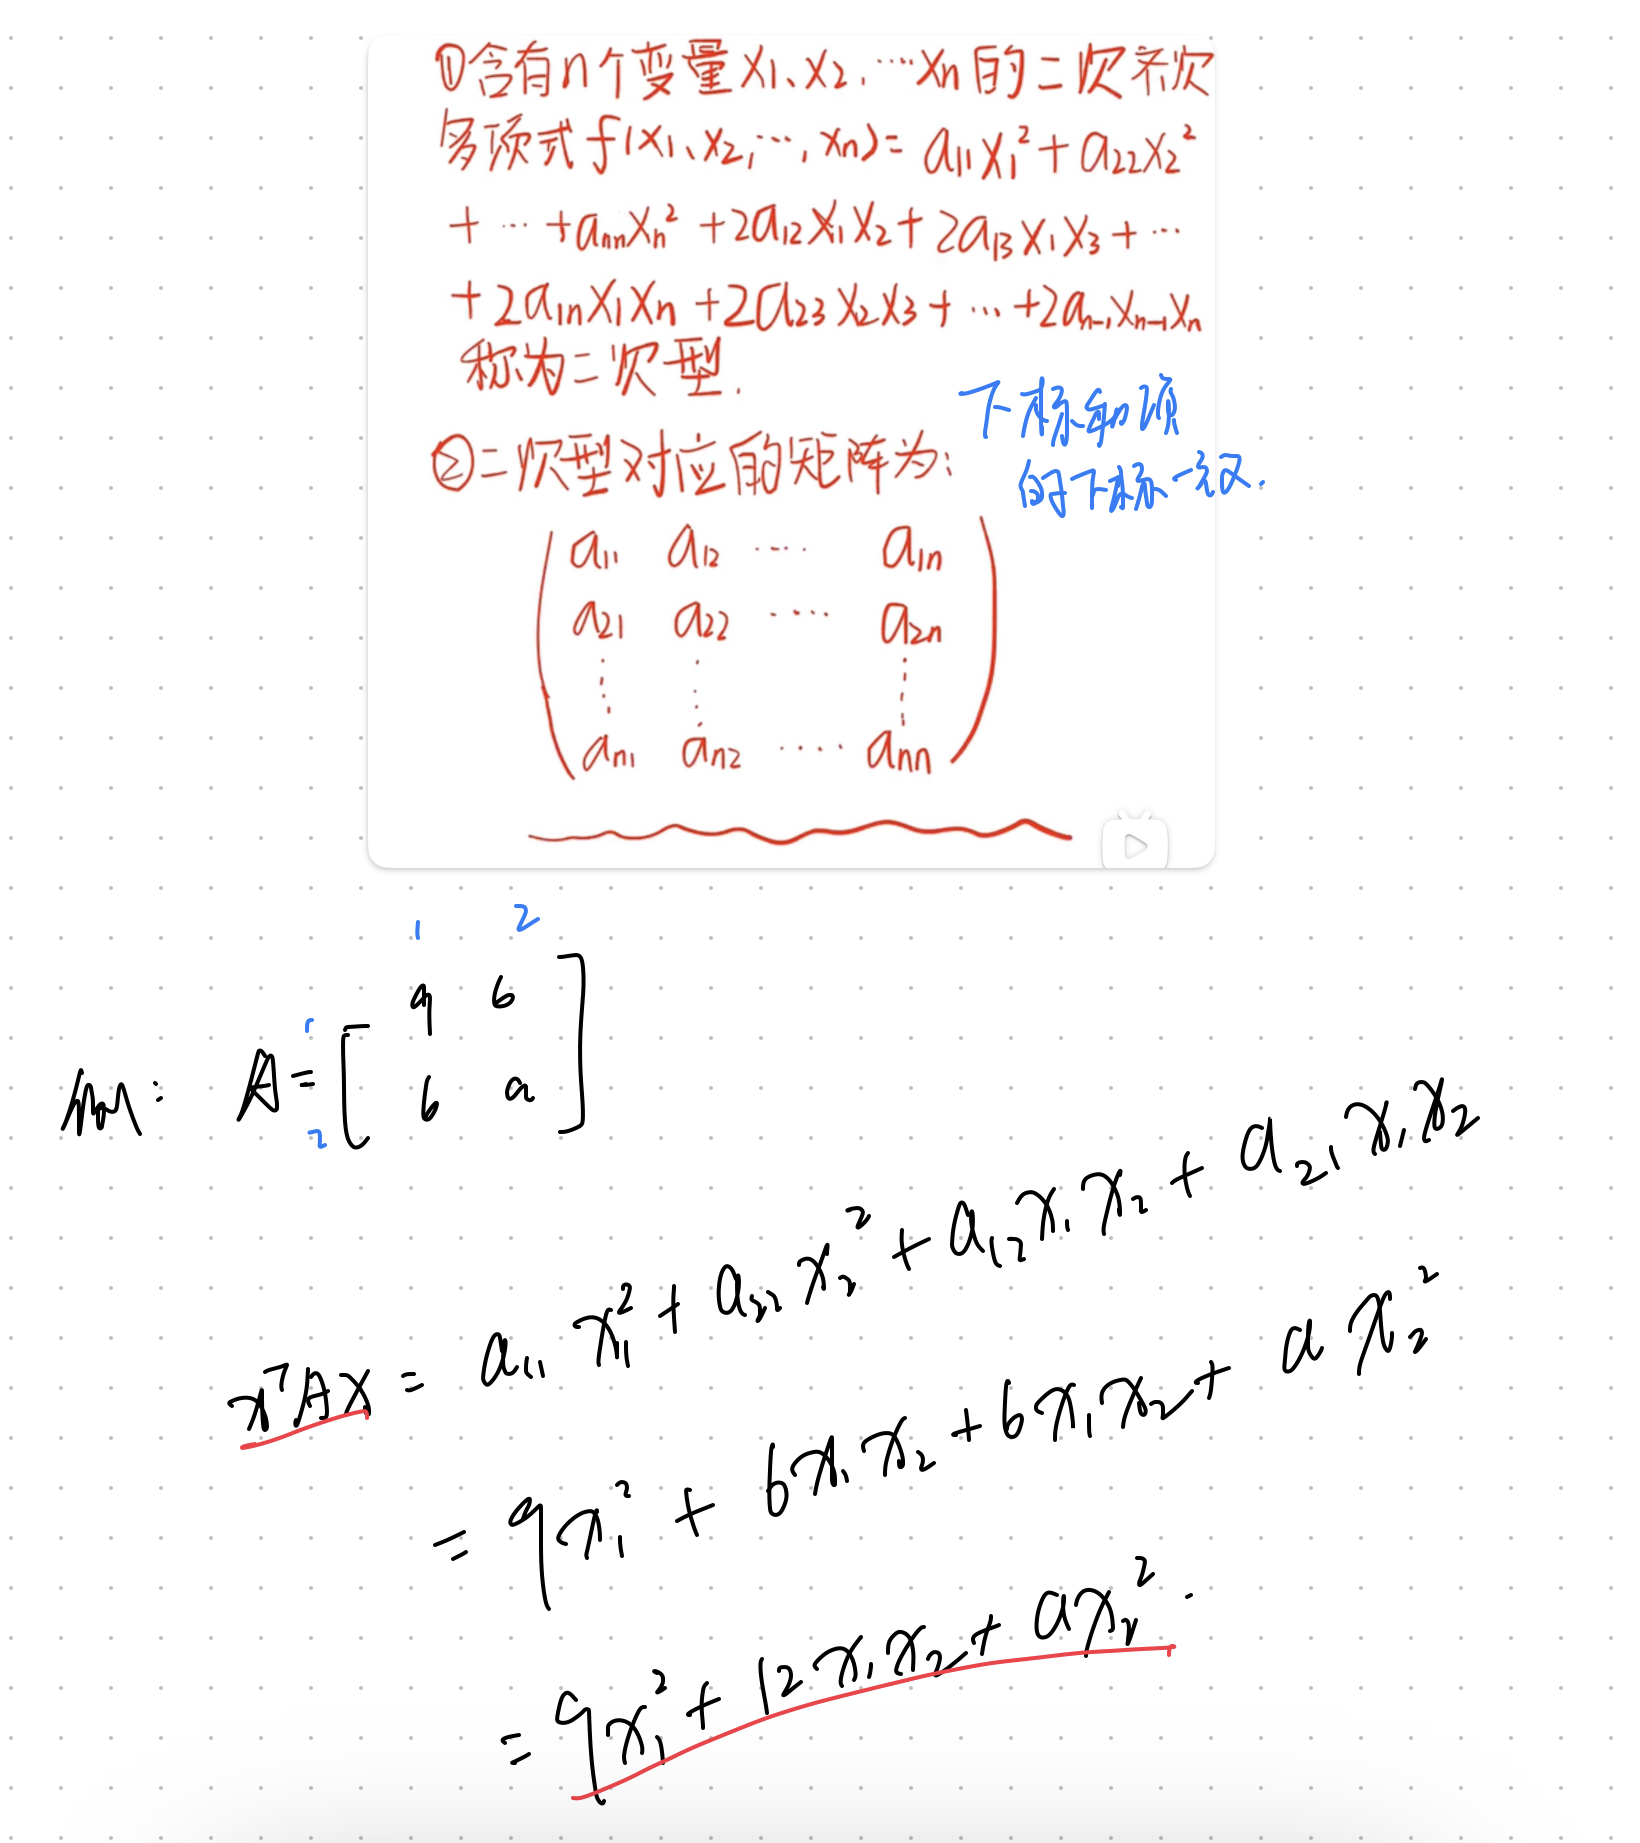
\includegraphics[width=1\linewidth]{lec6-7}\\
2, pred by this:\\
\includegraphics[width=1\linewidth]{lec6-8}\\

\subsection*{Example}
\includegraphics[width=1\linewidth]{lec6-10}\\


\subsection{Pred by leading principal minors}
\includegraphics[width=1\linewidth]{6-12}\\

\subsection{Conclusions}
1, Semi-definite matrix may be nonsingular, not as positive definite one.



\pagebreak
\section{Gram matrix $X^TX$}
Gram matrix is a special type of matrix
to describe the inner product relationships between sets of vectors. 
Specifically, if there is a set of vectors $[v1, v2, ..., vn]$, then the elements 
$G_{ij}$ of the Gram matrix G are the inner products of vectors $v_i$ and $v_j$, 
that is, $Gij = <vi, vj>$. The Gram matrix is semi-positive definite, and it is positive definite when the set of vectors is linearly independent.

\includegraphics[width=1\linewidth]{6-11}\\

\pagebreak
\section{Symmetric positive definite matrices, SPD}
\subsection{Definition of SPD}
A square matrix is SPD \textbf{iff}
it is \textbf{symmetric} and all its eigenvalues $\lambda$ are \textbf{positive},
that is $\lambda > 0$.\\
Note: \\
- Don't forget the 2nd part of the definition, sometimes useful to think in this way.\\
- This is an iff relationship.

\subsection*{Properties}
\textbf{1, Diagonal entries of SPD is positive.}\\
\\
Proof starting from the definition: Known that A is SPD, then
for all nonzero vector $u$, we have $\left\langle Au,u\right\rangle > 0$.
\noindent
Then, utilize identity matrix to extract an element of A. (MV Product, dot product view). Good enough.\\

\noindent
\textbf{2, SPD iff Each $A_k$ is SPD}\\
will fill this part later.\\

\noindent
\textbf{3, a conclusion}\\
will fill this part later.\\


\noindent
\textbf{4, If A is SPD, then for any nxk matrix X of rank k, the matrix $X^TAX$ is SPD.}\\
Memory:\\
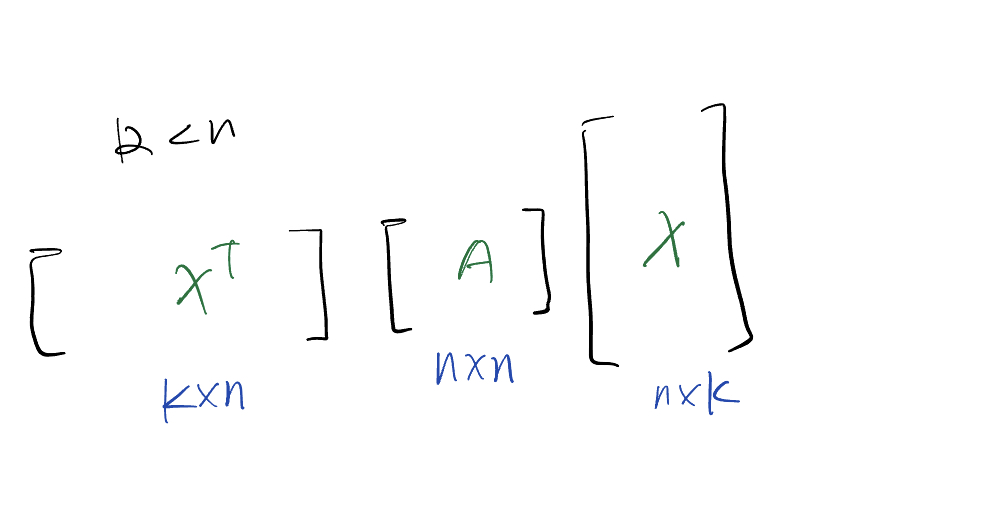
\includegraphics[width=1\linewidth]{lec6-1.jpg}
Proof (will use the notation of the inner product and def of SPD):\\




\subsection*{Application: Covariance Matrices in Statistics}


\pagebreak
\section{The $LDL^T$ Factorization from LU}
\subsection*{Theorem}
\includegraphics[width=1\linewidth]{lec6-5}\\

\noindent
For the LU Factorization, all we need is all $A_k$ matrices for k=1 to n-1 have to
be nonsingular. As A is SPD, implying that all $A_k$ matrices from k=1 to n are nonsingular.
Thus LU fac exists and is unique.\\

\noindent
Inverse of a Diagonal Matrix is easy to compute:\\
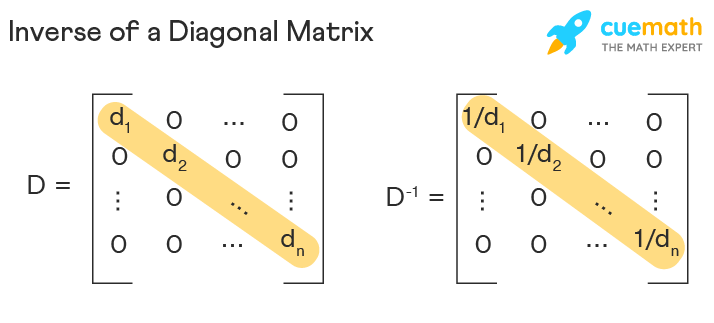
\includegraphics[width=1\linewidth]{lec6-2.png}

\noindent
Nice results because of symmetry

L is M

\noindent
Proof that $A = LU = LDL^T$\\

\noindent
Thus, a SPD matrix A could be written in this form: $A = LDL^T$
where L is a lower triangular matrix with 1s on the diagonal, and D is a diagonal matrix (of U).\\



\pagebreak
\section{The Cholesky Factorization GGT from LDLT}

GGT, scope of application: SPD matrices (??? what about semi-definte matrix???).\\

Diagonal of D shoud be positive so that we can take a square root to D to reach the Cholesky.\\
\\
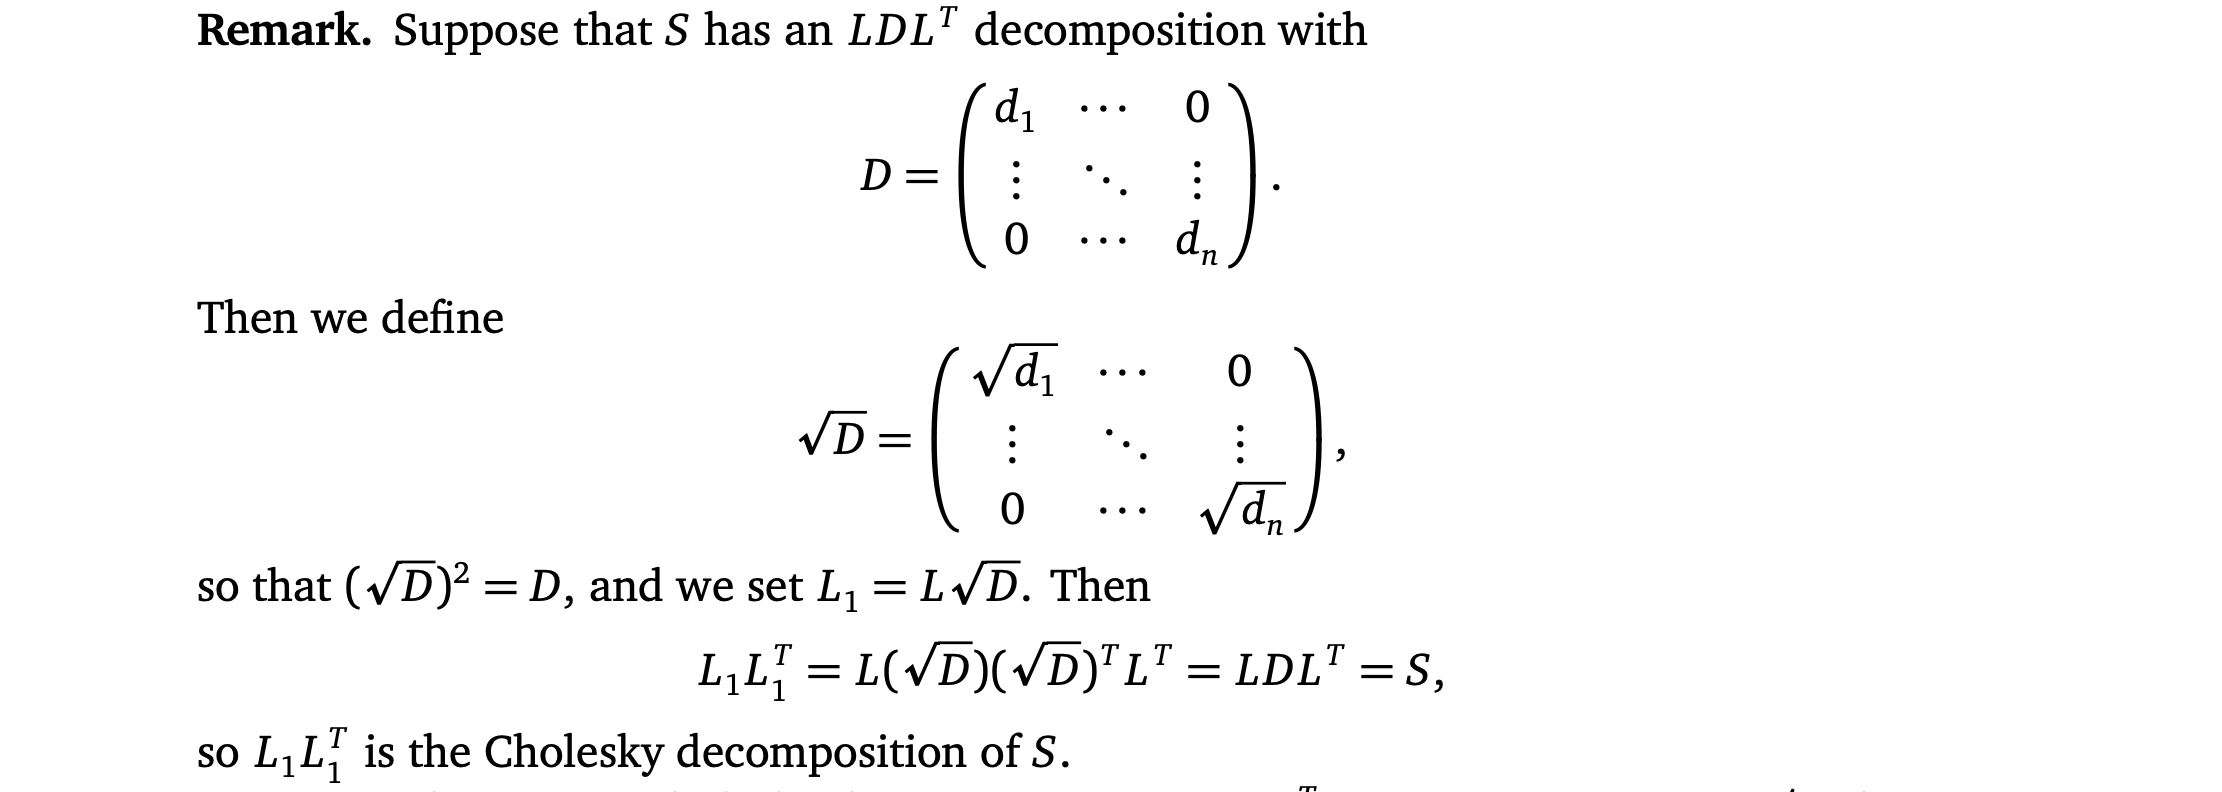
\includegraphics[width=1.5\linewidth]{lec6-3.png}\\
\\
\medskip
Proof: Diagonal of D shoud is positive


\noindent
What can we say about G? G is lower triangular

\noindent
The Cholesky: Any matrix that is SPD could be written as $A = GGT$ where G is a lower triangular matrix, and positive
entries on diagonal.\\

\pagebreak
\section{Algos of LDLT and GGT}
\subsection*{row-oriented LDLT}
Idea: Adapted from Gaussian but just work on upper part of the matrix because of symmetry because
the working matrix A(k+1:n, k+1:n) in standard LU remains symmetric. See graph below:\\
\includegraphics[width=1\linewidth]{lec6-4.jpg}\\


\noindent
Proof: A(k+1:n, k+1:n) is symmetric (induction argument).\\
\\
\noindent
What is the cost(FLOPs) of this algo?\\
Cost of standard LU:\\
Suppose k's index starting from 0, then in standard LU decomposition, when clearing
the 1st col, each row replacement invoves n-1 multiplications (scale piv row) and n-1 substraction (update
curr row), 2(n-1) flops in total. Hence, when k increase, problem size decrese, it takes $2(n-2)^2$ flops
to clear the 2nd col etc.. Thus, we have:\\
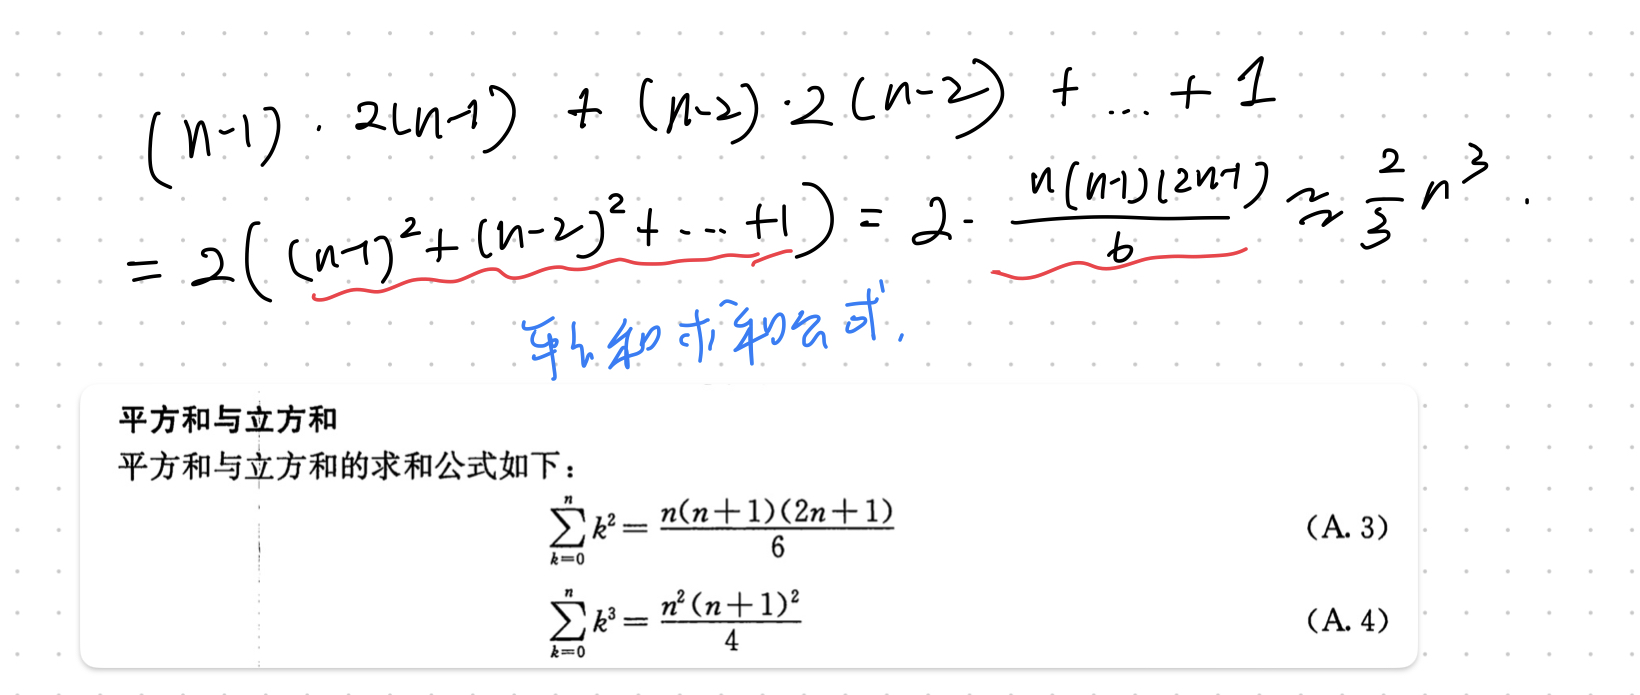
\includegraphics[width=1\linewidth]{lec6-6}\\

\noindent
Cost of LDLT (just half of LU): $\frac{1}{2} * \frac{2}{3}*n^3 = \frac{1}{3}*n^3$\\


\noindent
Rank 1 update: You're updating the matrix by something like $uv^T$ where u and v are the same.\\

\noindent
\subsection*{2, row GGT, outer product form}

\noindent
\subsection*{3, column-oriented LDLT}

\end{document}